According to the trainless accuracy predictor published by IBM \cite{Scheidegger2018}, the validation accuracy for the first few epochs of a smaller network are linearly related to the final test accuracy. If their experiment is solid, then we could expect it works for relative accuracy as well, for a particular dataset. Also, we want to know if this works for other network, like DenseNet121 as well. We plotted the results in Figure \ref{Fig.training_trend} with our training history data to analysis this hypothesis. We didn't use CIFAR20 and CIFAR40 history because we want to focus on large datasets.

The result is not exactly linear in our case. The shape is more like part of a arc instead. However, if we take a closer look at the data which achieves a relative accuracy larger than 0.9, then the curve is more close to a linear line, especially for CIFAR10.
\section{Subset Selection Framework}
\begin{figure}[H]
\centering  
\subfigure[Epoch 5]{
\label{Fig.sub.a1}
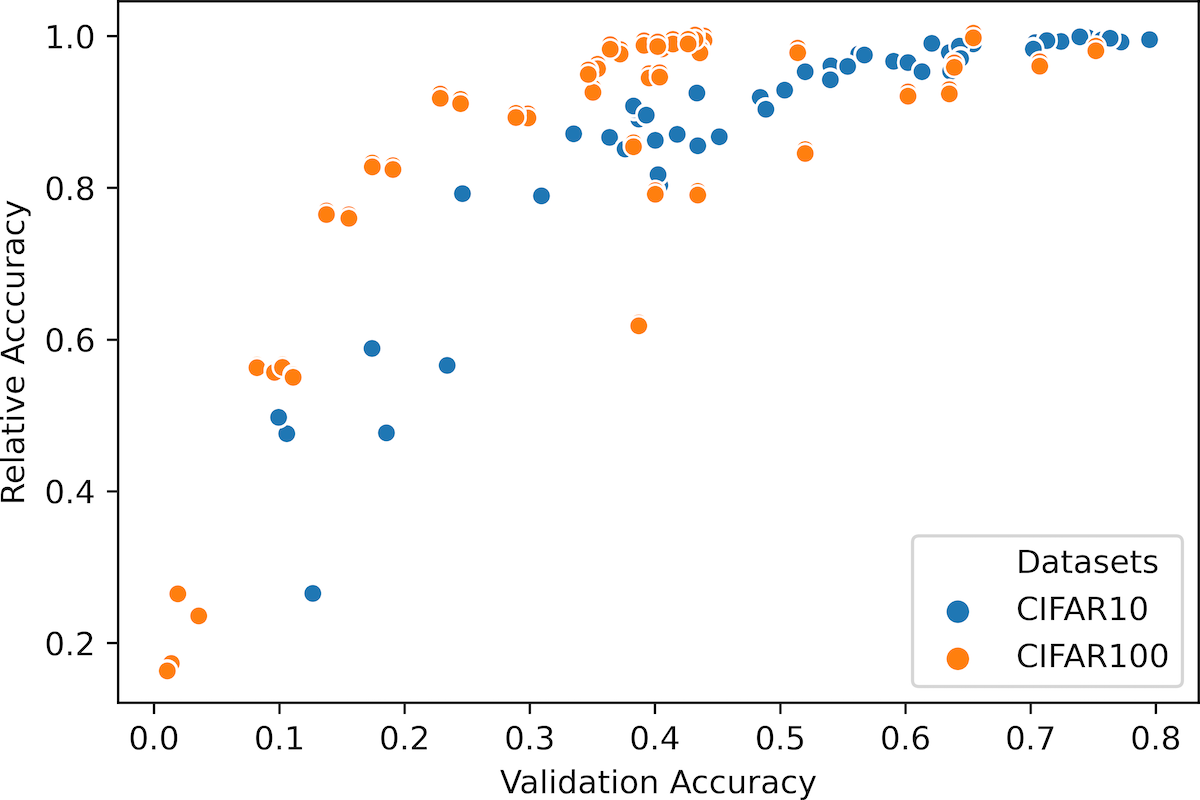
\includegraphics[width=0.32\textwidth]{src/valid_relative_5.png}}
\subfigure[Epoch 7]{
\label{Fig.sub.a1}
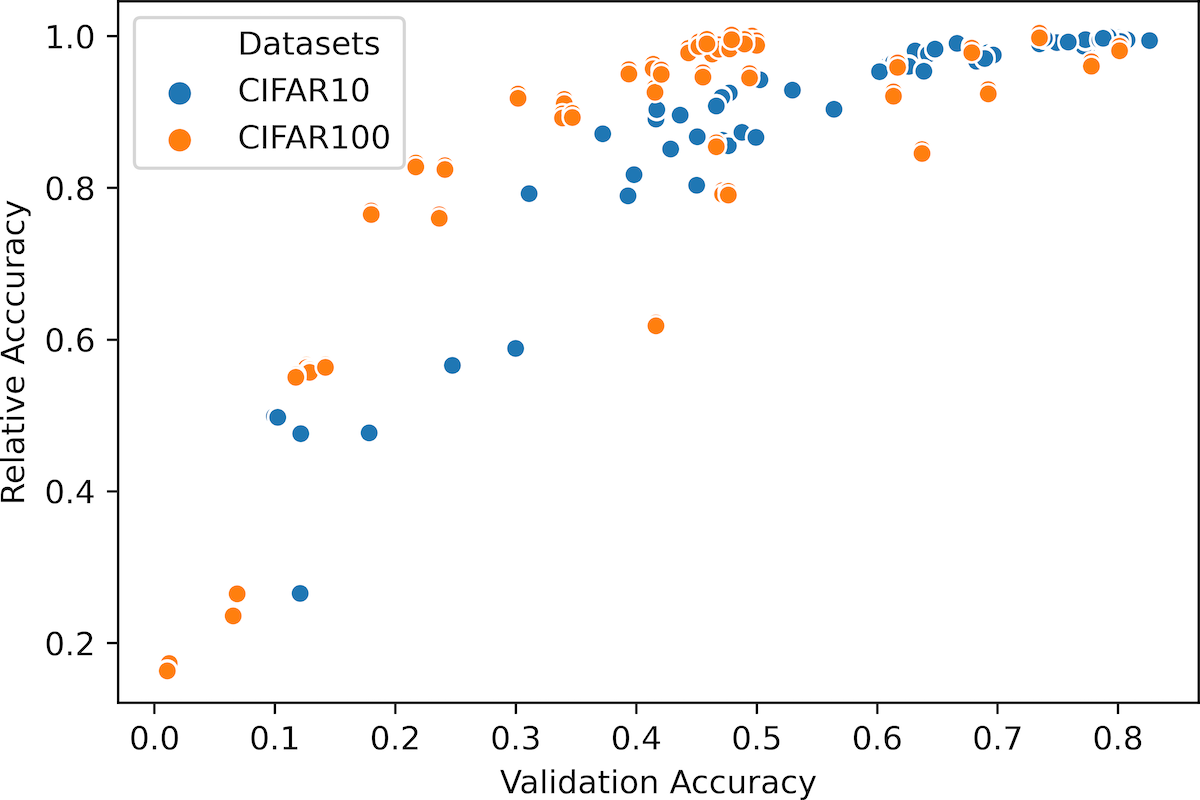
\includegraphics[width=0.32\textwidth]{src/valid_relative_7.png}}
\subfigure[Epoch 9]{
\label{Fig.sub.a2}
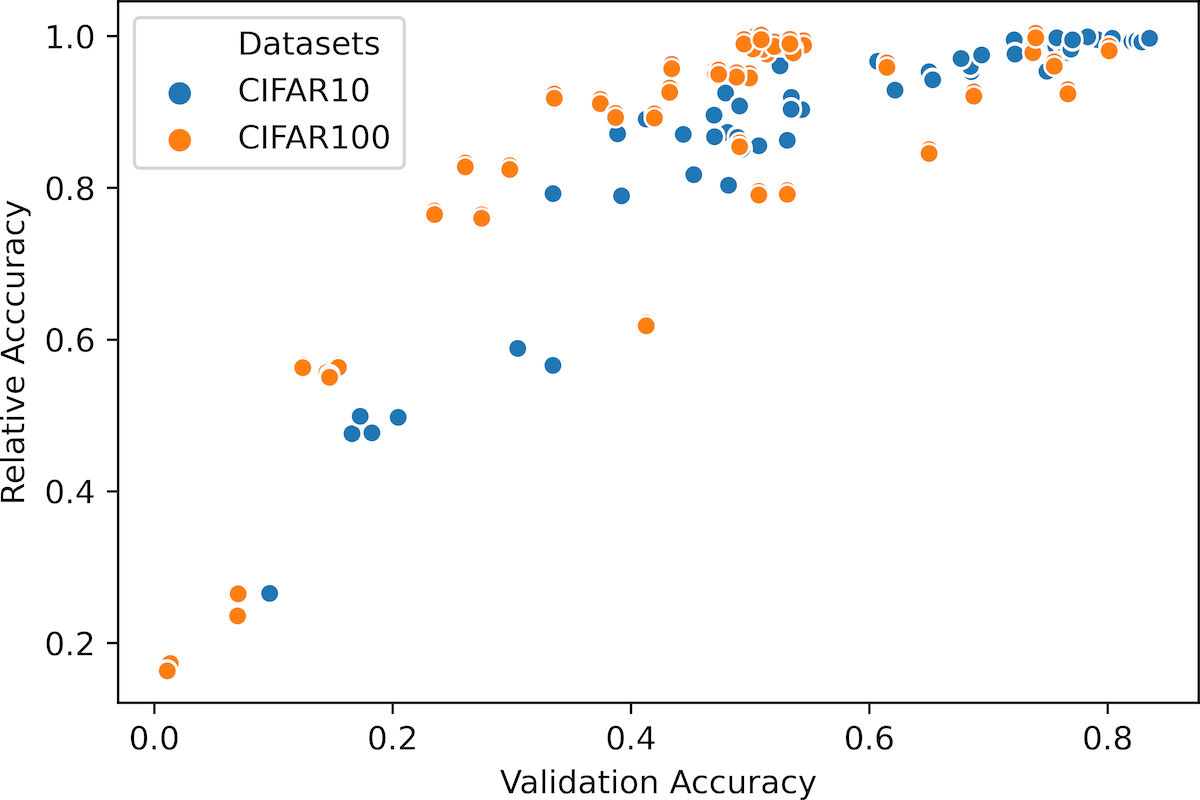
\includegraphics[width=0.32\textwidth]{src/valid_relative_9.png}}
\caption{The linear relationship between the validation accuracy and the final relative accuracy achieved}
\label{Fig.training_trend}
\end{figure}

We also explored the logit transformation method recommended by \cite{Kornblith2018}, who claims that we can have a better linear shape. In Figure \ref{Fig.training_trend}, we can see that this is true. However, this is still not good enough because we also want to link it the hyper-parameter.

\begin{figure}[H]
\centering  
\subfigure[Epoch 5]{
\label{Fig.sub.a1}
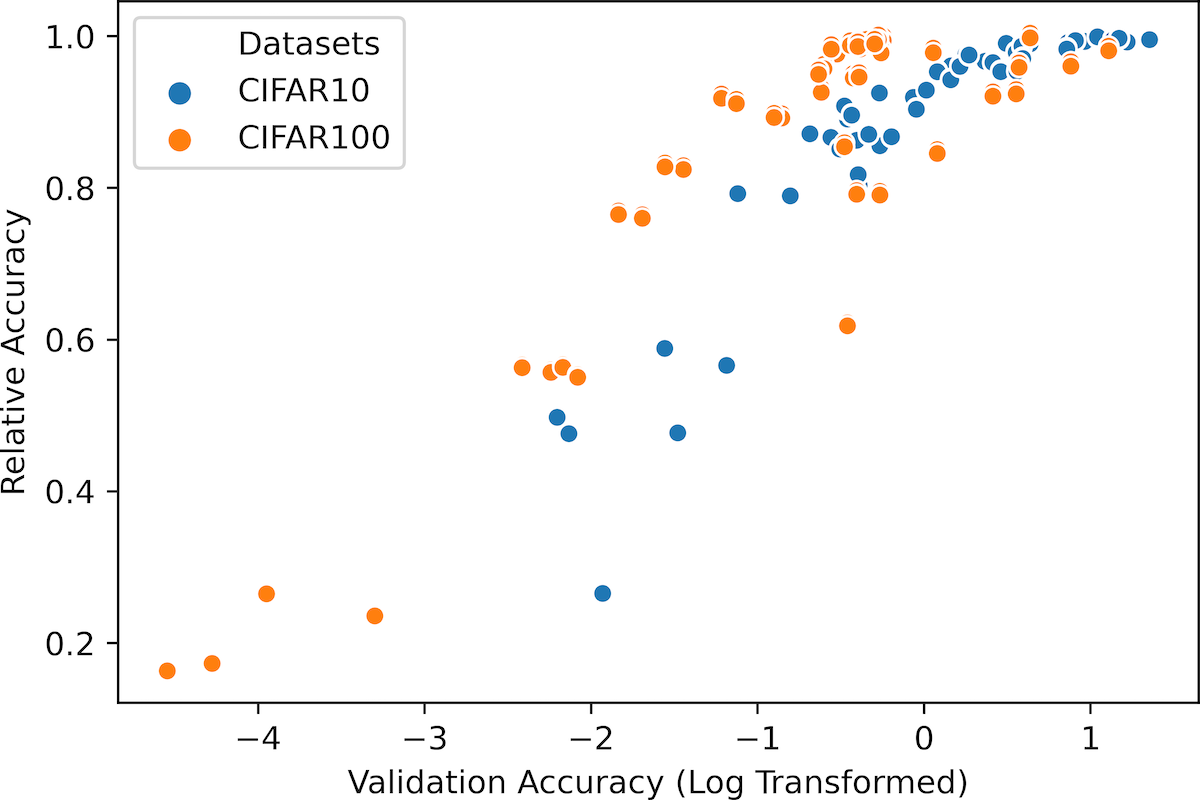
\includegraphics[width=0.32\textwidth]{src/valid_log_relative_5.png}}
\subfigure[Epoch 7]{
\label{Fig.sub.a1}
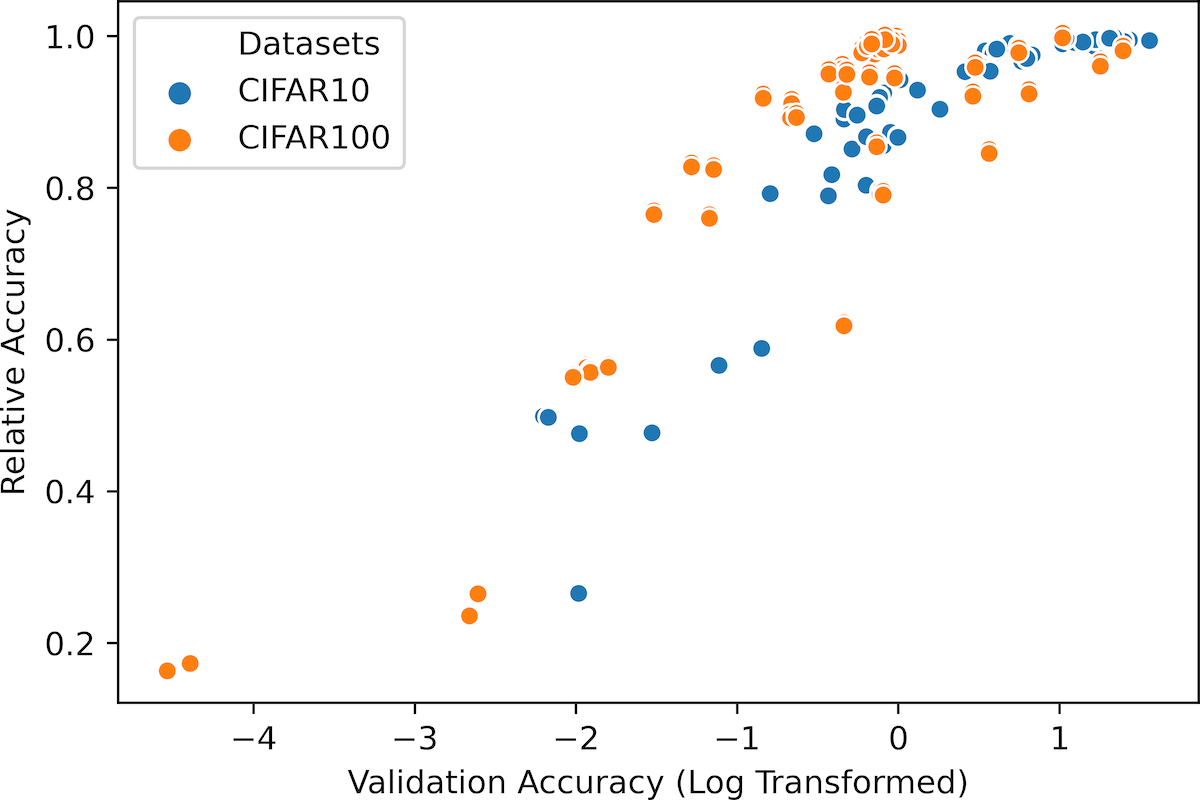
\includegraphics[width=0.32\textwidth]{src/valid_log_relative_7.png}}
\subfigure[Epoch 9]{
\label{Fig.sub.a2}
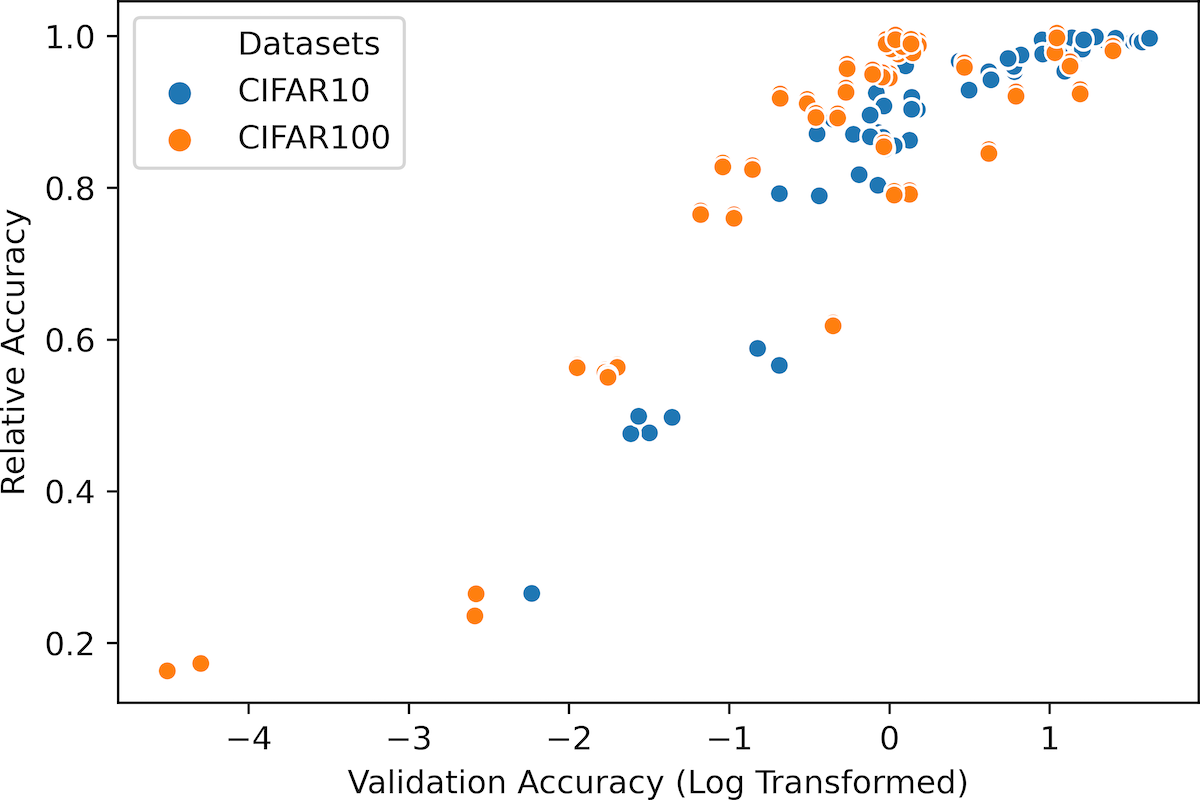
\includegraphics[width=0.32\textwidth]{src/valid_log_relative_9.png}}
\caption{The linear relationship between the validation accuracy and the final relative accuracy achieved}
\label{Fig.training_trend}
\end{figure}

Therefore, we trained a simple logistic regression model which takes the first 10 epochs' validation accuracy and the first 5 epochs whole dataset validation accuracy as the input. By selecting only samples with accuracy larger than 90\%, we got a good results shown in Figure \ref{Fig.training_trend}.

\begin{figure}[H]
\centering  
\subfigure[CIFAR10 train]{
\label{Fig.sub.a1}
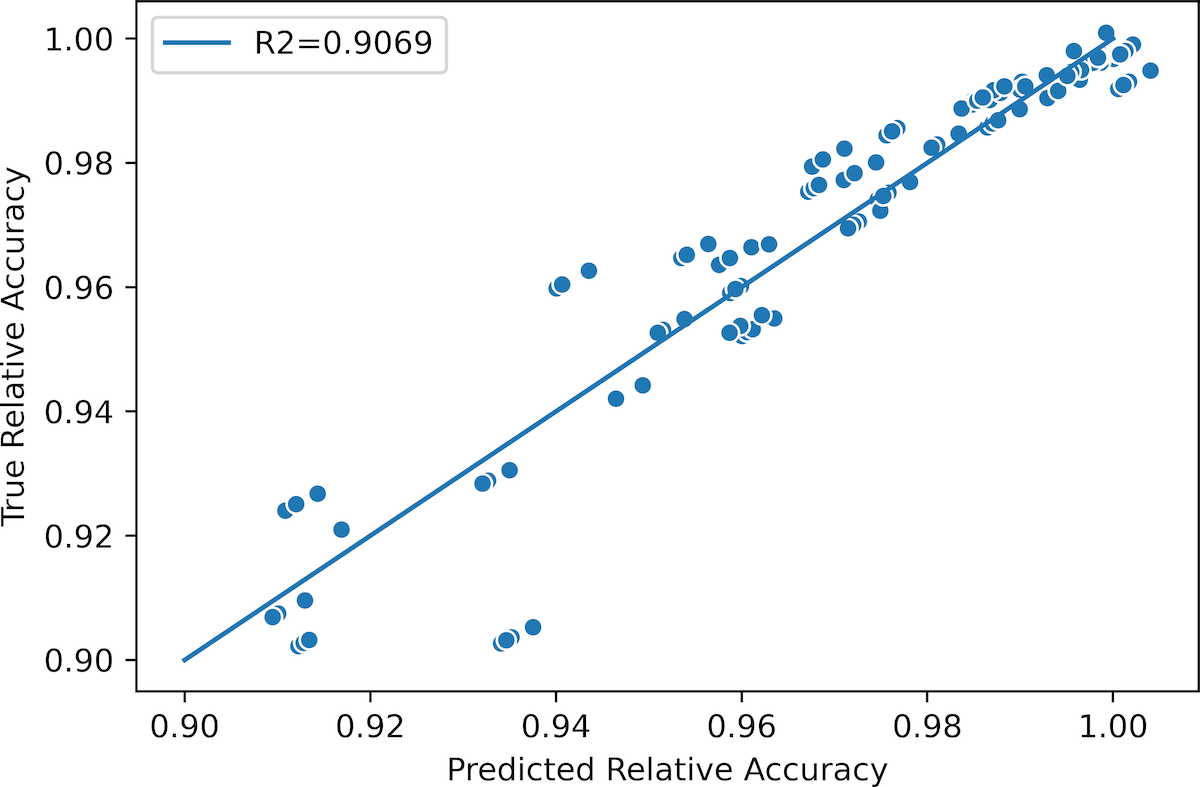
\includegraphics[width=0.45\textwidth]{src/cifar10_tradeoff.png}}
\subfigure[CIFAR10 test]{
\label{Fig.sub.a2}
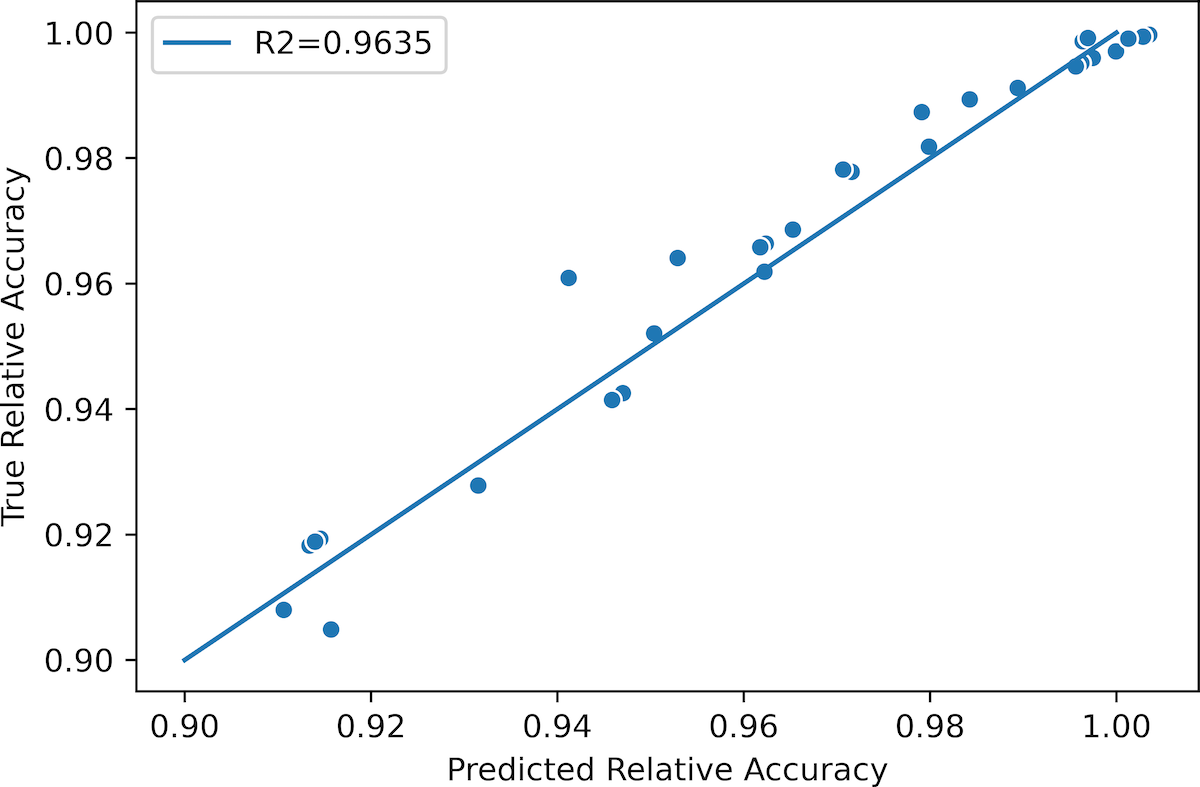
\includegraphics[width=0.45\textwidth]{src/cifar10_tradeoff_test.png}}

\subfigure[CIFAR100 train]{
\label{Fig.sub.a1}
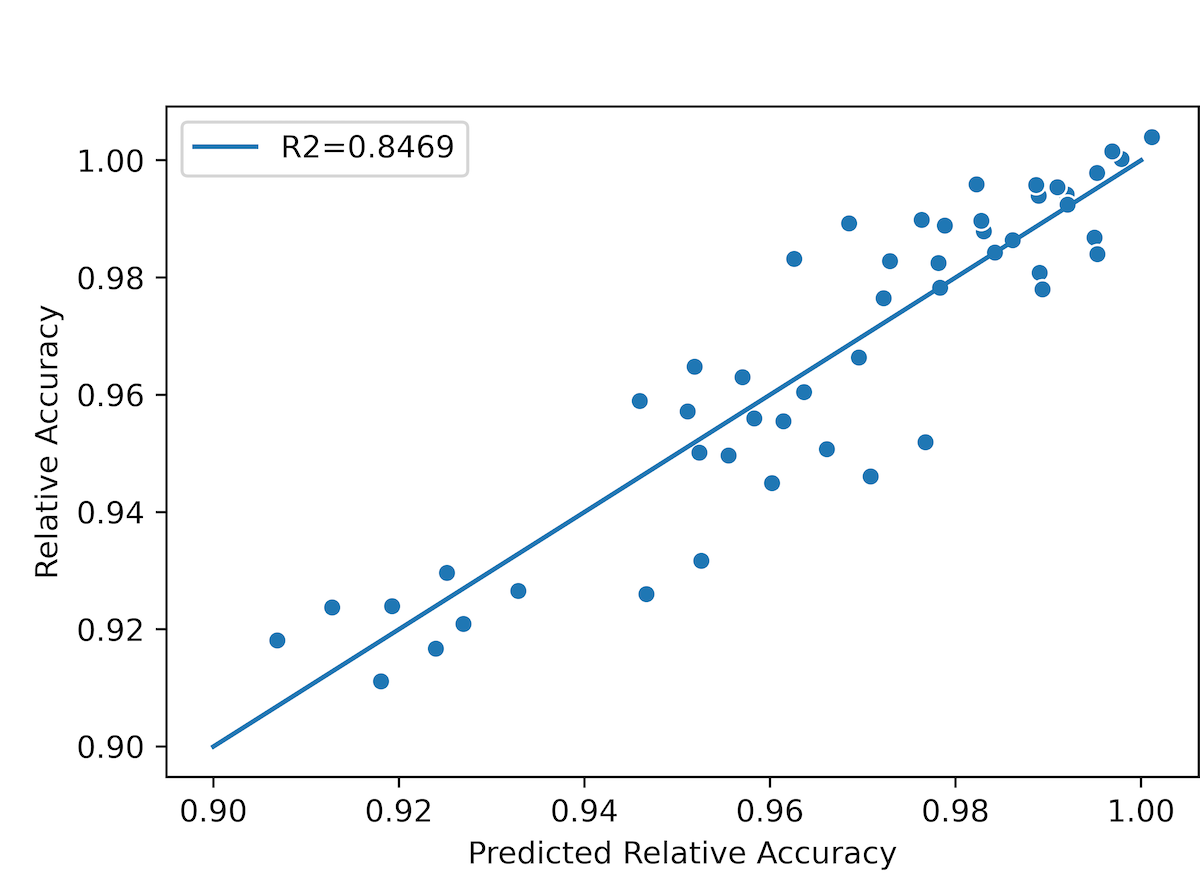
\includegraphics[width=0.45\textwidth]{src/cifar100_tradeoff.png}}
\subfigure[CIFAR100 test]{
\label{Fig.sub.a2}
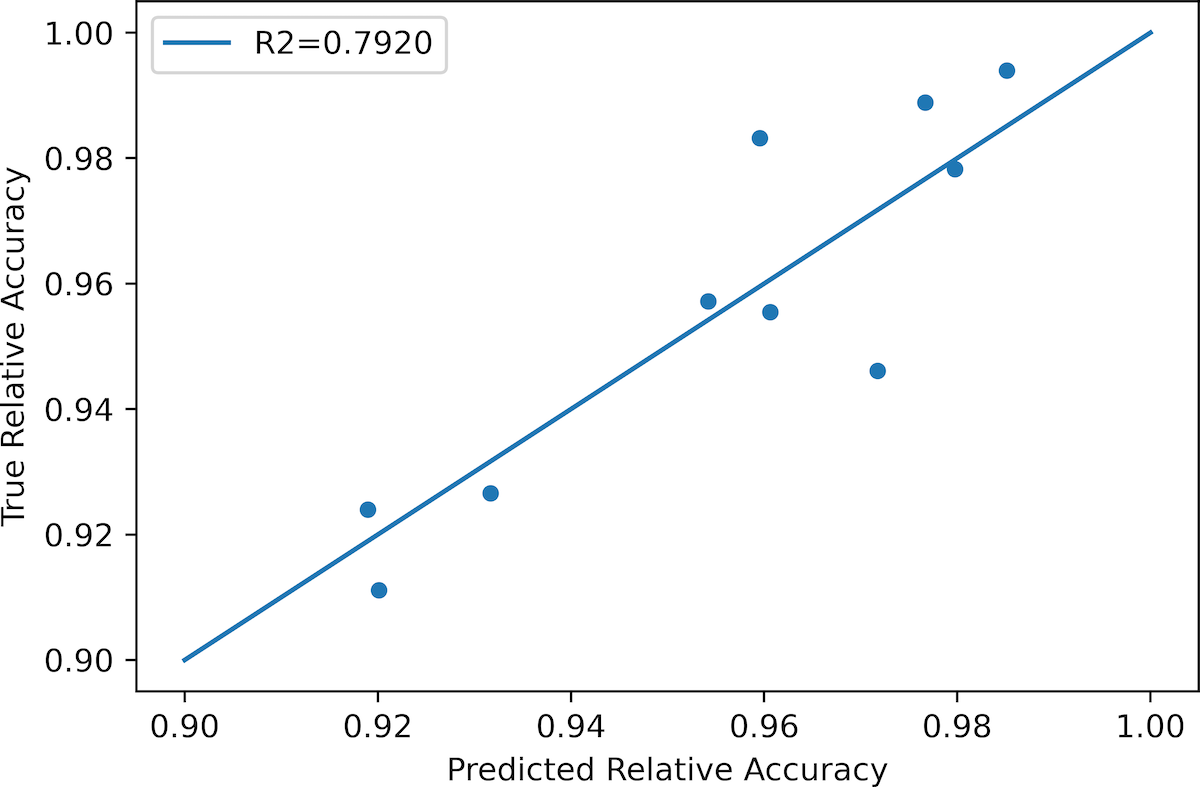
\includegraphics[width=0.45\textwidth]{src/cifar100_tradeoff_test.png}}
\caption{The linear model for CIFAR10 and CIFAR100 to predict the relative accuracy}
\label{Fig.training_trend}
\end{figure}

Then we train with subsets selected from CIFAR10 and CIFAR100 for only 100 